%%%%%%%%%%%%%%%%%%%%%%%%%%%%%%%%%%%%%%%%%%%%%%%%%%%%%%%
%                   File: OSAmeetings.tex             %
%                  Date: March 21, 2007  MSD          %
%                                                     %
%     For preparing LaTeX manuscripts for submission  %
%       submission to OSA meetings and conferences    %
%                                                     %
%       (c) 2007 Optical Society of America           %
%%%%%%%%%%%%%%%%%%%%%%%%%%%%%%%%%%%%%%%%%%%%%%%%%%%%%%%

\documentclass[letterpaper,10pt]{article}
\usepackage{osameet2}

%% standard packages and arguments should be modified as needed

%%\usepackage{amsmath,amssymb}
\usepackage{indentfirst}
\setlength{\parindent}{2em}
    

%\usepackage[pdftex,colorlinks=true,bookmarks=false,citecolor=blue,urlcolor=blue]{hyperref} %pdflatex
\usepackage[dvips,colorlinks=false,bookmarks=false,citecolor=blue,urlcolor=blue]{hyperref} %latex w/dvips

\begin{document}
\title{Flattened Switching Node with Flexible Co-propagation of Quantum and Optical Signals}
%%\title{Flattened Flexible Non-blocking Switching Node with Quantum and Classic Optic Coexistence}
\author{Pandeng Li, Yongmei Sun}
\address{State Key Laboratory of Information Photonics and Optical Communications, School of Information and Telecommunication Engineering, BUPT Beijing, China, 100876}
\email{ymsun@bupt.edu.cn}
\begin{abstract}
\noindent We propose a flattened switching node with flexible co-propagation of quantum and optical signal that could combine the quantum key distribution network and Optical network into one. and we exhibit a stable experimental platform that could show the practical value of this structure.
%%Quantum key distribution provides an unconditional physical layer for secure communication.Study on switching and large-scale Networking problems in Quantum Communication could promote QKD communication to industrialization and practical. The current quantum switching nodes can only handle the wavelength of a specific bandwidth and have a strong constraint on the path of the transmission. And the spectrum reuse rate is very low. So it can't meet the demands of build large-scale network. This paper will present a WSS-based flattened flexible and non-blocking switching node that could support quantum communication and classic optical communication at the same time with multi-granularity.
\end{abstract}
\ocis{(060.5565) Quantum communications, (060.1810)Co-switching devices}

\section{Introduction}
Quantum key distribution provides an unconditional physical layer for secure communication\cite{ToliverPaul} and uses non-orthogonal coded single photon states, such as single photon polarization, phase or angular momentum, to provide secure information. These all can be transmitted and switched as same as optical signal in the fiber. So far, the study on point-to-point co-fiber transmission for QKD communication has been quite mature. More and more researchers have turned into studying large-scale and multi-user QKD network based on optical network. In 2003, Paul Toliver made an experiment of an optical switching system for QKD communication based on the 4x4 2-D MEMS switch array and reached a transmission distance more than 10 km\cite{ToliverPaul}. But this system couldn't support the case of the co-switching of multiple wavelengths that have different destination. In 2010, Shuang Wang et al. of USTC proposed a wavelength-saving quantum switching device composed of a three-port looper and WDM\cite{WangShuang} and it has low power loss and high stability.  However this scheme adopted the real-time full connection and increased the complexity of the network. The schemes above neither considered to integrate the quantum network into the existing optical network. This paper will present an flattened switching node scheme supporting the co-propagation of quantum signal and optical signal, the node is based on WSS and coupler and could provide abilities of flexible spectrum allocation and non-blocking switching.

\section{Difference between quantum communication and classical optical communication}
To integrate quantum communication with optical communication, we should consider similarities and differences between quantum signal and optical signal. The quantum signal can't be amplified, it needs the link loss to be extremely low, while the optical signal is not sensitive to the link loss. When passing through the beam splitter, quantum signal only appear in one branch of the beam splitter at a specific probability, while optical signal appear in all branch of the beam splitter at a specific ratio of the input power. In the process of QKD, the delay time between quantum signal and synchronization signal has an important effect on key generate rates.the synchronization signal is needed to have the same path with quantum signal on the link layer to keep the signal synchronized. However, the classical optical signal doesn't require additional synchronization signal. Meanwhile,quantum signal is extremely weak and is very easy to be disturbed by optical signals of other channels, so it is very important to consider the effects of optical signals on quantum signals when they are co-propagated. 

\section{Flattened switching node based on WSS}
We makes full use of the characteristics of WSS: (a)Flexgrid Dynamic Channel Width Control; (b)Flexgrid Dynamic Attenuation Control; (c)Channel plans are configurable 'on-the-fly'. These make WSS meet the needs of co-switching of quantum signal with optical signal. the switching node structure is showed in figure \ref{fig:switching_node_structure}.
\begin{figure}[htbp]
  \centering
  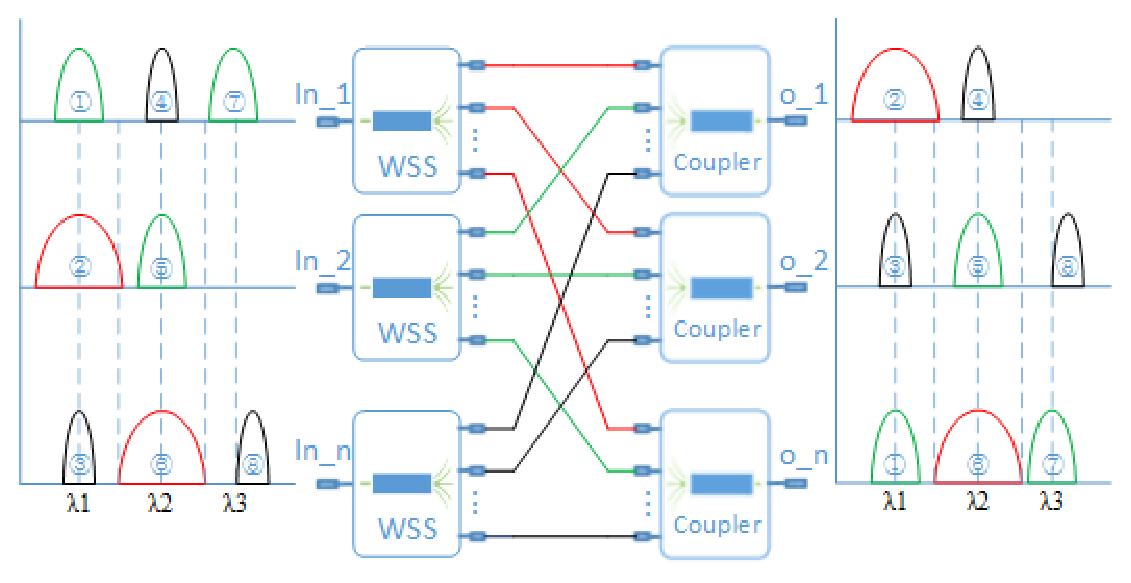
\includegraphics[width=8.3cm]{swtiching_node_struct}
  \caption{Switching Node Structure.} \label{fig:switching_node_structure}
\end{figure}
The switch node only have two kinds of optical devices, WSS and coupler. It has the characteristics of flexible grid, multi-granularity, low loss, non-blocking. so it could switch signal with variety of bandwidth Simultaneously and could achieve "Packet Routing" that the signals who have same destination but different center wavelength and bandwidth could always passing through the same optical fiber path. Based on this switching node, we could also design a wavelength allocation algorithm to reduce the impairment on the quantum channels induced by four-wave mixing (FWM). When expanding node's degree, it doesn't increase the device cascade, Since it's attenuation remains stable, approximately 3.5 dB under current technical conditions.
For optical signal, There is only one constraint that the signals couldn't overlap in the spectrum when switched to the same port. In figure \ref{fig:switching_node_structure}, wave 2 and wave 6 have different center wavelength, but their spectrum have a little intersection, so they can't be switched to the same port. For quantum signal, we could compute the channels that FWM sit on according to the current optical signal passing the node, and make quantum signal stay away from these channels to reduce the interference induced by FWM when allocating the quantum signal channel. In the past studies, someone have proposed switching node based on WDM and OXC, and multi-granularity switching node of three-layers based on DWDM, CWDM and OXC. The comparisons of these three structures show that the flattened switching node we proposed has lower loss.

\begin{figure}[!htb]
   \begin{minipage}{0.48\textwidth}
     \centering
     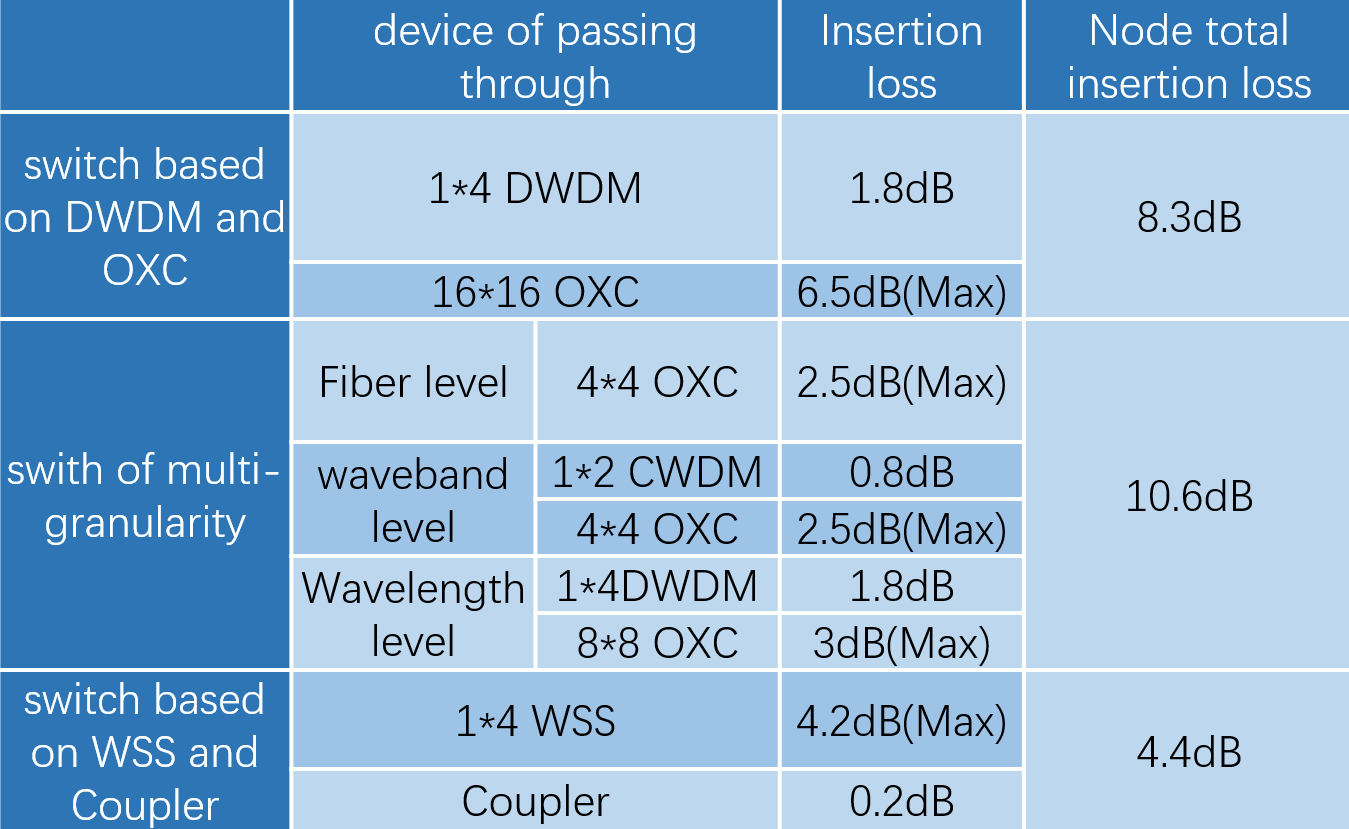
\includegraphics[height= 4cm,width=.9\linewidth]{comparison_of_three_kind_of_nodes}
     \caption{Comparison of Insertion Loss} \label{Fig:comparison_of_loss}
   \end{minipage}\hfill
   \begin{minipage}{0.48\textwidth}
     \centering
     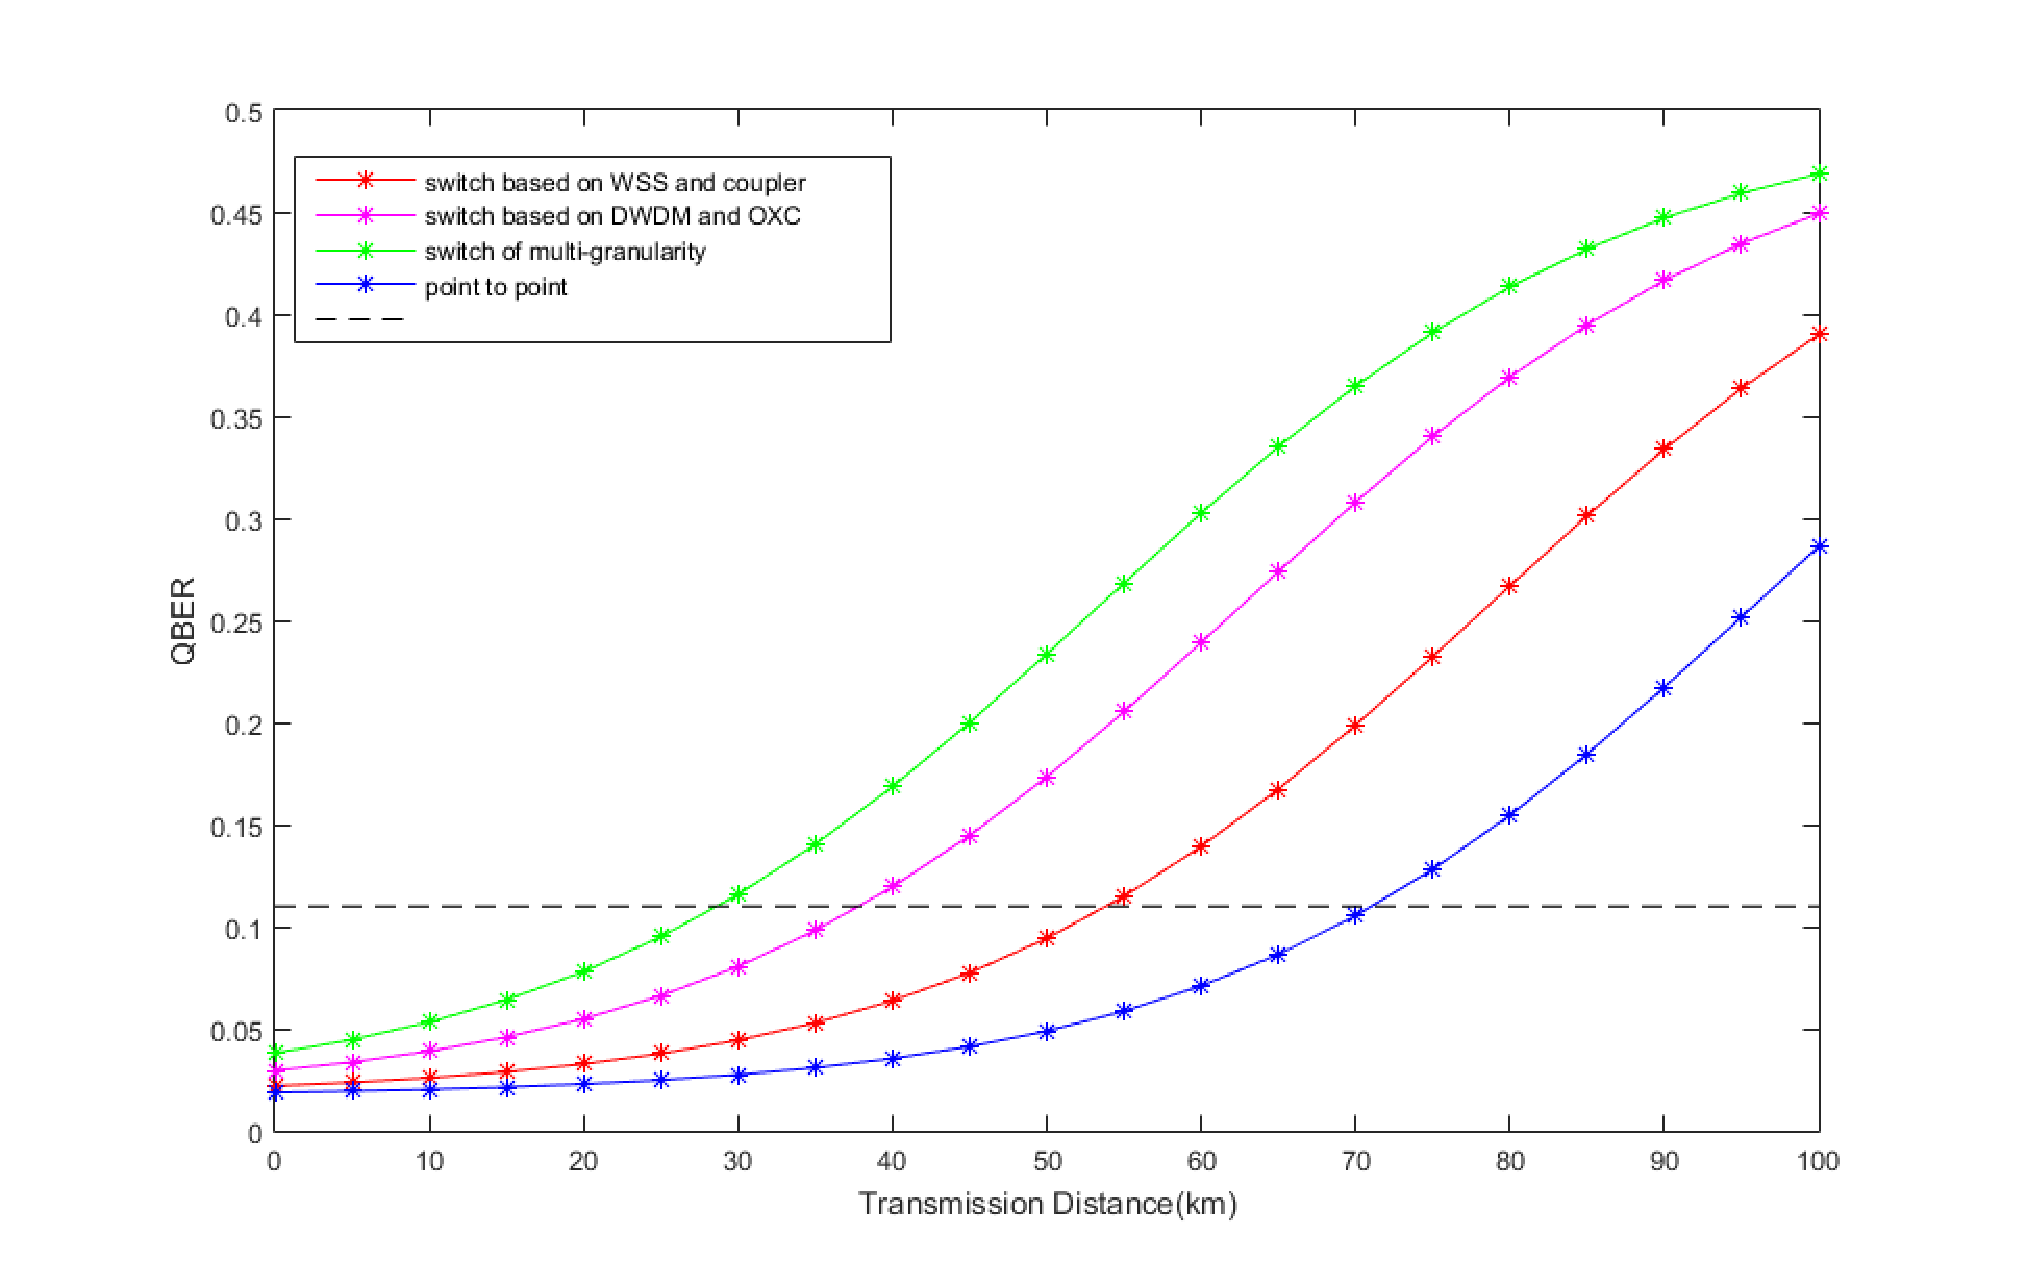
\includegraphics[height= 4cm,width=.9\linewidth]{transmission_distance_vs_QBER_of_three_nodes_2}
     \caption{Transmission Distance vs QBER} \label{Fig:comparison_of_rate}
   \end{minipage}
\end{figure}

\section{Experiment setup}
Our experimental implementation is composed of quantum transmitter/receiver, optical transmitter/receiver and the switching node as figure \ref{Fig:experiment_of_switching_node} show.
\begin{figure}
 \centering
 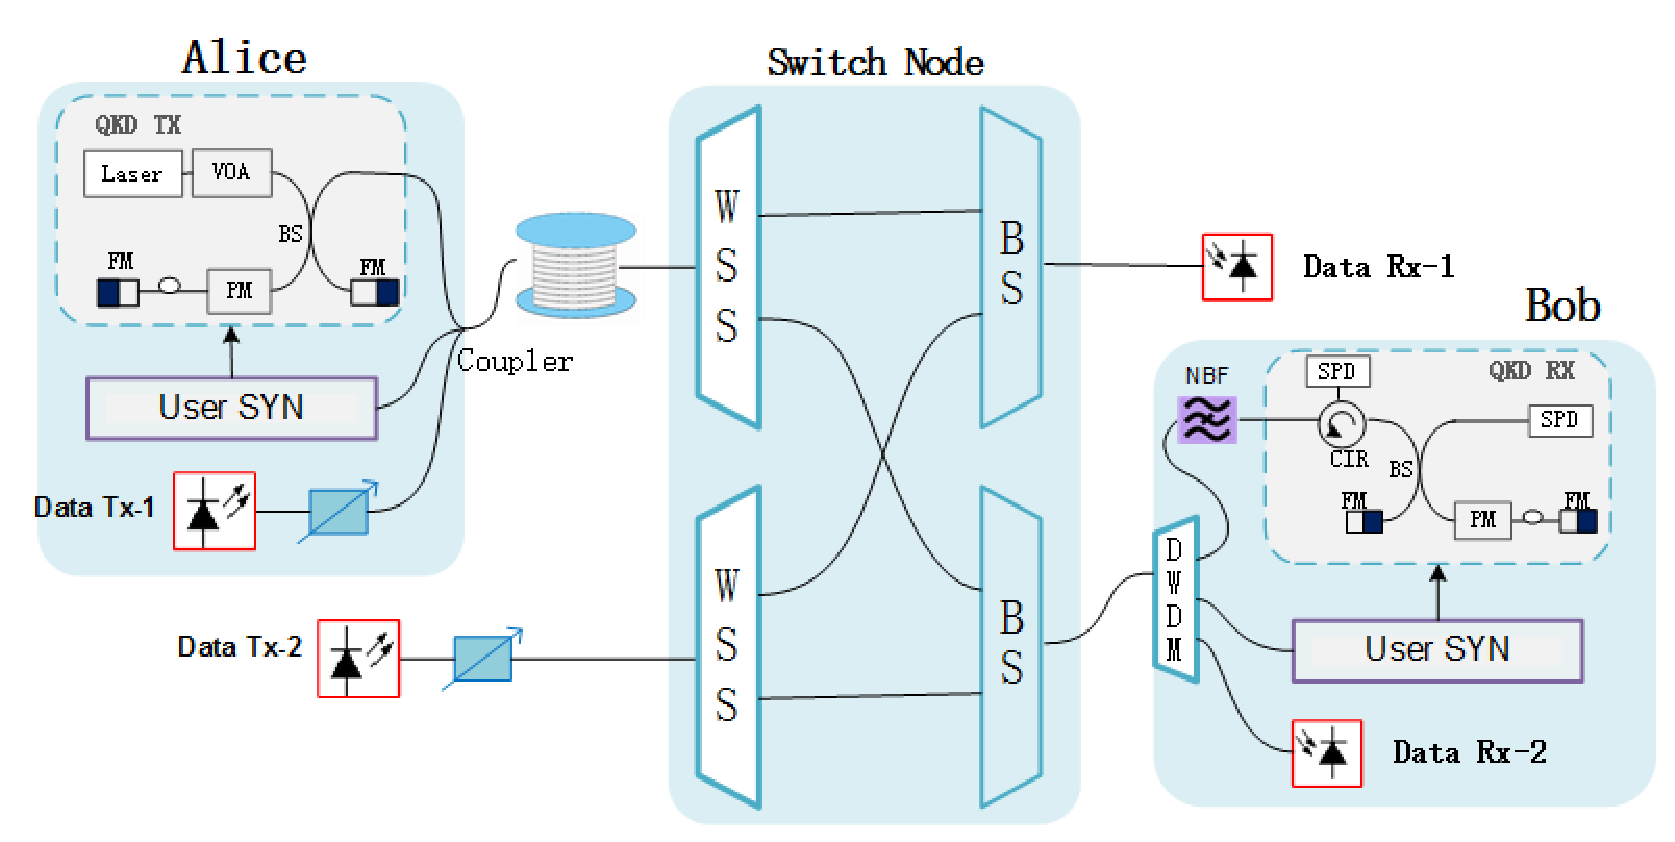
\includegraphics[height= 4cm,width=.8\linewidth]{experiment_of_switching_node}
 \label{Fig:experiment_of_switching_node}
 \caption{experiment setup of coexistence switching node}
\end{figure}
Alice have abilities of sending the quantum signal, quantum sync signal and optical signal. Bob could receive and parse these three kind of signals. QKD transmitter consists of a pulsed light source (LS), a Faraday-Michelson interferences(FM) containing a phase modulator (PM) and a variable optical attenuator(VOA). QKD receiver has one more signal photon detector(SPD). Since it is difficult to create true single photon pulses, a pulsed 1553.73nm laser diode (1-ns pulse width) with 500MHz repetition rate is followed by variable optical attenuator to approximate single photon generation. In order to detect the quantum signal within the appropriate time, we need a signal to synchronize the time of detection and set it's center wavelength 1529.99nm. There are two 1550nm Optical waves for sending large data as text, image, video etc. When performing quantum communication, there are a lot base selection information needed to be send on the public network. Since the switching node is unidirectional, if we make the public network through the quantum switching node and switched by switching node, we need to build two switch nodes. In account cost consideration, we build another public network without switching  that connect Alice and Bob Directly. In this experiment, we set up three sets of contrast experiments. (a) Point-to-point quantum communication experiment; (b) Only quantum communication passes through the switching node; (c) Quantum communication and classical optical communication pass through the switching node at the same time. The experimental results of the three experiments are shown in the following figure.
\begin{figure}[!htb]
   \begin{minipage}{0.48\textwidth}
     \centering
     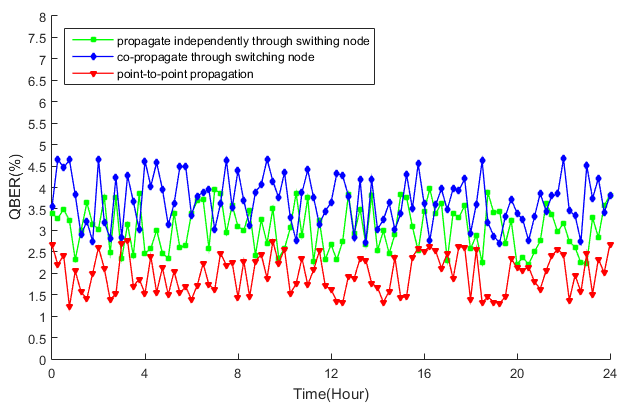
\includegraphics[width=.9\linewidth]{qber_experiment}
     \caption{QBER performance for 24 hours} \label{Fig:comparison_of_loss}
   \end{minipage}\hfill
   \begin{minipage}{0.48\textwidth}
     \centering
     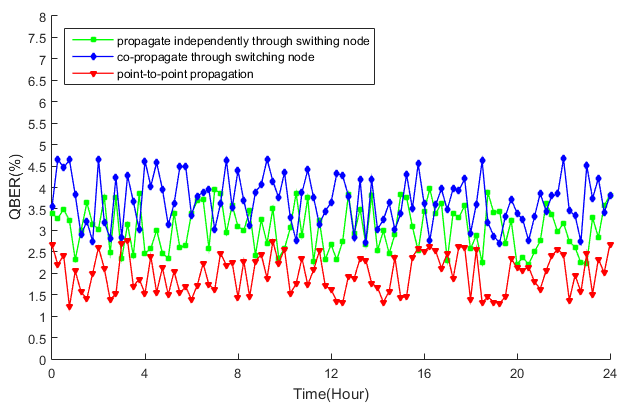
\includegraphics[width=.9\linewidth]{qber_experiment}
     \caption{Key generation rates performance for 24 hours} \label{Fig:comparison_of_rate}
   \end{minipage}
\end{figure}
figure \ref{Fig:comparison_of_loss} and \ref{Fig:comparison_of_rate} show 24 hours of continuous operation. the results show that the co-propagation switching could be realized by the switching node we proposed and the QBER and key generation rate is acceptable. 

\section{Conclusions}
We propose a flattened switching node with flexible co-propagation of quantum and classical opticals signal. This architecture support flexiable spectrum allocation and the experiment demostrate that this node could support the co-propagation swithcing of quantum signal with optical signal.
%%We proposed a flattened flexible non-blocking switching node with quantum and classic optic coexistence, this architecture could be compatible with the switch of quantum signals and classical optical signals,  quantum communication optical network and the integration of the classic optical network to provide the basis, which provides the foundation for the integration of quantum communication optical network and classical optical network.

\begin{thebibliography}{99}

\bibitem{ToliverPaul} Toliver, Paul, et al. "Experimental investigation of quantum key distribution through transparent optical switch elements." IEEE Photonics Technology Letters 15.11 (2003): 1669-1671.

\bibitem{YongmeiSun} Sun, Yongmei, et al. "Reduction of FWM noise in WDM-based QKD systems using interleaved and unequally spaced channels." Chinese Optics Letters 14.6 (2016): 060602.

\bibitem{WangShuang} Wang, Shuang, et al. "Field test of wavelength-saving quantum key distribution network." Optics letters 35.14 (2010): 2454-2456.

%%\bibitem{Jensen} Jensen, Richard, and Andrew Lord. "Novel non-blocking low loss scalable WSS architecture." Optical Fiber communication/National Fiber Optic Engineers Conference, 2008. OFC/NFOEC 2008. Conference on. IEEE, 2008.

\bibitem{NiuJianing} Niu, Jianing, et al. "A Novel Scheme of Integrating QKD in WDM-PON." Asia Communications and Photonics Conference. Optical Society of America, 2016.

\end{thebibliography}
\end{document}
